\chapter{Регионы России}
\label{ch:oblast-of-Russia}
Эта глава книги посвящена исследованию в Викиданных регионов России. 
Отметим, что регионы России включают в себя множество земель разного 
типа: области, республики, края и другие. Именно эти разнотипные регионы 
и были исследованы. Был построен граф субъектов России, граничащих 
с зарубежными странами (граф соседей), а также нарисована карта, 
на которой отмечена численность населения отдельных регионов. Оценка 
степени заполненности свойства Викиданных <<граничит с>> (shares border with) 
показала, что у каждого субъекта России эти данные заполнены полностью. Были построены две карты, на которых цветом обозначены граничные регионы и пограничные страны.
Читатель познакомится с компьютерной обработкой Викиданных и визуализацией 
информации о регионах России.

\label{question:q_subjects_of_Russia_3}
\marginnote{О флаге какого субъекта идет речь:
<<Флаг этого субъекта представляет собой прямоугольное полотнище с отношением ширины к длине 2:3, красного цвета с двусторонним изображением в верхнем ближнем к древку углу основного элемента герба этого субъекта~--- развёрнутого к древку Святого \href{https://ru.wikipedia.org/wiki/Георгий_Победоносец}{Георгия Победоносца}. См. ответ \ref{answer:subjects_of_Russia_3} на с.~\pageref{answer:subjects_of_Russia_3}.}

\section{Экземпляры объекта <<Области России>>}

Для построения списка всех областей России нам потребуются объект 
\wdqName{<<области России>>}{835714} и свойство \wdProperty{31}{<<экземпляры>>} 
(листинг~\ref{lst:oblast-of-Russia}).

\begin{lstlisting}[ language=SPARQL, numbers=none,
                    caption={\href{https://w.wiki/4D2V}{Список всех областей России}\protect\footnotemark},
                    label=lst:oblast-of-Russia,
                    texcl 
                    ]
# List of oblasts of Russia
SELECT ?region ?regionLabel
WHERE
{
  ?region wdt:P31 wd:Q835714. # instance of "oblast of Russia"
  SERVICE wikibase:label {bd:serviceParam wikibase:language "ru"}
}
\end{lstlisting}%
\footnotetext{Получено 48 записей в 2017 году и 46 записей в 2021 году. Ссылка на SPARQL-запрос: \href{https://w.wiki/4D2V}{https://w.wiki/4D2V}}

В Викиданных больше всего свойств в России и в мире у \wdqName{Ленинградской}{2191} и \wdqName{Калининградской областей}{1749}, по 43 свойства\autocite{Russia_prowd}. Число свойств для России и мира одинаковое, так как и для России, и для мира это одни и те же объекты.

Областями России с наименьшим числом свойств по данным сервиса ProWD оказались: \href{http://www.wikidata.org/entity/Q3129}{Орловская область} (31 свойство), \href{http://www.wikidata.org/entity/Q3178}{Курская область} (31 свойство), \href{http://www.wikidata.org/entity/Q5851}{Новосибирская область} (32 свойство).


\section{Субъекты Российской Федерации}

Построим список всех субъектов России. Для этого выберем следующие объекты в Викиданных: республики, края, области, города федерального значения, автономные области и автономные округа (листинг~\ref{lst:subjects-of-Russia}).

%\footnotetext{
\marginnote{Используемые в запросах объекты:
\begin{itemize}
	\item\wdqName{<<области России>>}{835714};
	\item\wdqName{<<республики России>>}{41162};
	\item\wdqName{<<города федерального значения России>>}{183342};
	\item\wdqName{<<края России>>}{831740};
	\item\wdqName{<<автономные области России>>}{309166};
	\item\wdqName{<<автономные округа России>>}{184122};
	\item\wdqName{<<бывшая административно-территориальная единица>>}{19953632}.
\end{itemize}
Используемое свойство \wdProperty{31}{<<экземпляры>>}
}

\begin{lstlisting}[ language=SPARQL, numbers=none,
                    caption={\href{https://w.wiki/4D2R}{Список всех субъектов России}\protect\footnotemark},
                    label=lst:subjects-of-Russia,
                    texcl 
                    ]
# List of `instances of` "subjects of Russia" 
SELECT ?subject ?subjectLabel ?typeLabel
WHERE
{  
  VALUES ?type {wd:Q835714   # Oblast of Russia
                wd:Q41162    # Republic of Russia
                wd:Q183342   # Federal city of Russia
                wd:Q831740   # Krai of Russia
                wd:Q309166   # Autonomus oblast of Russia
                wd:Q184122}  # Autonomus okrug of Russia
  ?subject wdt:P31 ?type.  # Selecting the type of object
  SERVICE wikibase:label { bd:serviceParam wikibase:language "ru"}
}
\end{lstlisting}%
\footnotetext{Получено 85 записей в 2017 году и 86 записей в 2021 году. Ссылка на SPARQL-запрос: \href{https://w.wiki/4D2R}{https://w.wiki/4D2R}. В 2021 году в список субъектов добавился город федерального значения Байконур на правах аренды комплекса <<Байконур>>.}

Для построения скрипта~\ref{lst:subjects-of-Russia} и для проверки полученных результатов нужна следующая информация:
\begin{itemize}
  \item По данным Конституции Российской Федерации Россия состоит из 85 субъектов — республик, краёв, областей, городов федерального значения, автономной области, автономных округов.
  \item В этой задаче не учитываются субъекты, которые на текущий момент времени не входят в состав РФ (например, \wdqName{Читинская область}{182902}), поскольку они не являются экземплярами объектов \wdqName{<<области России>>}{835714}, \wdqName{<<республики России>>}{41162}, \wdqName{<<города федерального значения России>>}{183342}, \wdqName{<<края России>>}{831740}, \wdqName{<<автономные области России>>}{309166}, \wdqName{<<автономные округа России>>}{184122}, а относятся к объекту \wdqName{<<бывшая административно-территориальная единица>>}{19953632}. (Получаем 86 объекта после выполнения SPARQL-запроса, представленного на листинге~\ref{lst:subjects-of-Russia}). 
  \item По данным категории <<\href{https://ru.wikipedia.org/wiki/Субъекты_Российской_Федерации}{Субъекты Российской Федерации}>> Русской Википедии существует 85 субъектов РФ.
  \item По данным категории <<\href{https://ru.wikipedia.org/wiki/en:Federal_subjects_of_Russia}{Federal subjects of Russia}>> Английской Википедии так же существует 85 субъектов РФ.
\end{itemize}


\section{Соседние субъекты}

Построим граф соседних субъектов России по свойству \wdProperty{47}{shares border with} (листинг~\ref{lst:sharesBorderWith-oblast-of-Russia}).

\label{question:q_subjects_of_Russia_1}
\marginnote{Назовите регион России, расположенный на северо-западе России и образованный в \num{1920} году. Он граничит с Ленинградской, Вологодской, Архангельской и Мурманской областью. Также граничит с Финляндией на западе.
Выберите среди следующих флагов флаг этого региона. См. ответ \ref{answer:subjects_of_Russia_1} на с.~\pageref{answer:subjects_of_Russia_1}.}
\begin{marginfigure}[0.0cm]
{
	\setlength{\fboxsep}{0pt}%
	\setlength{\fboxrule}{1pt}%
	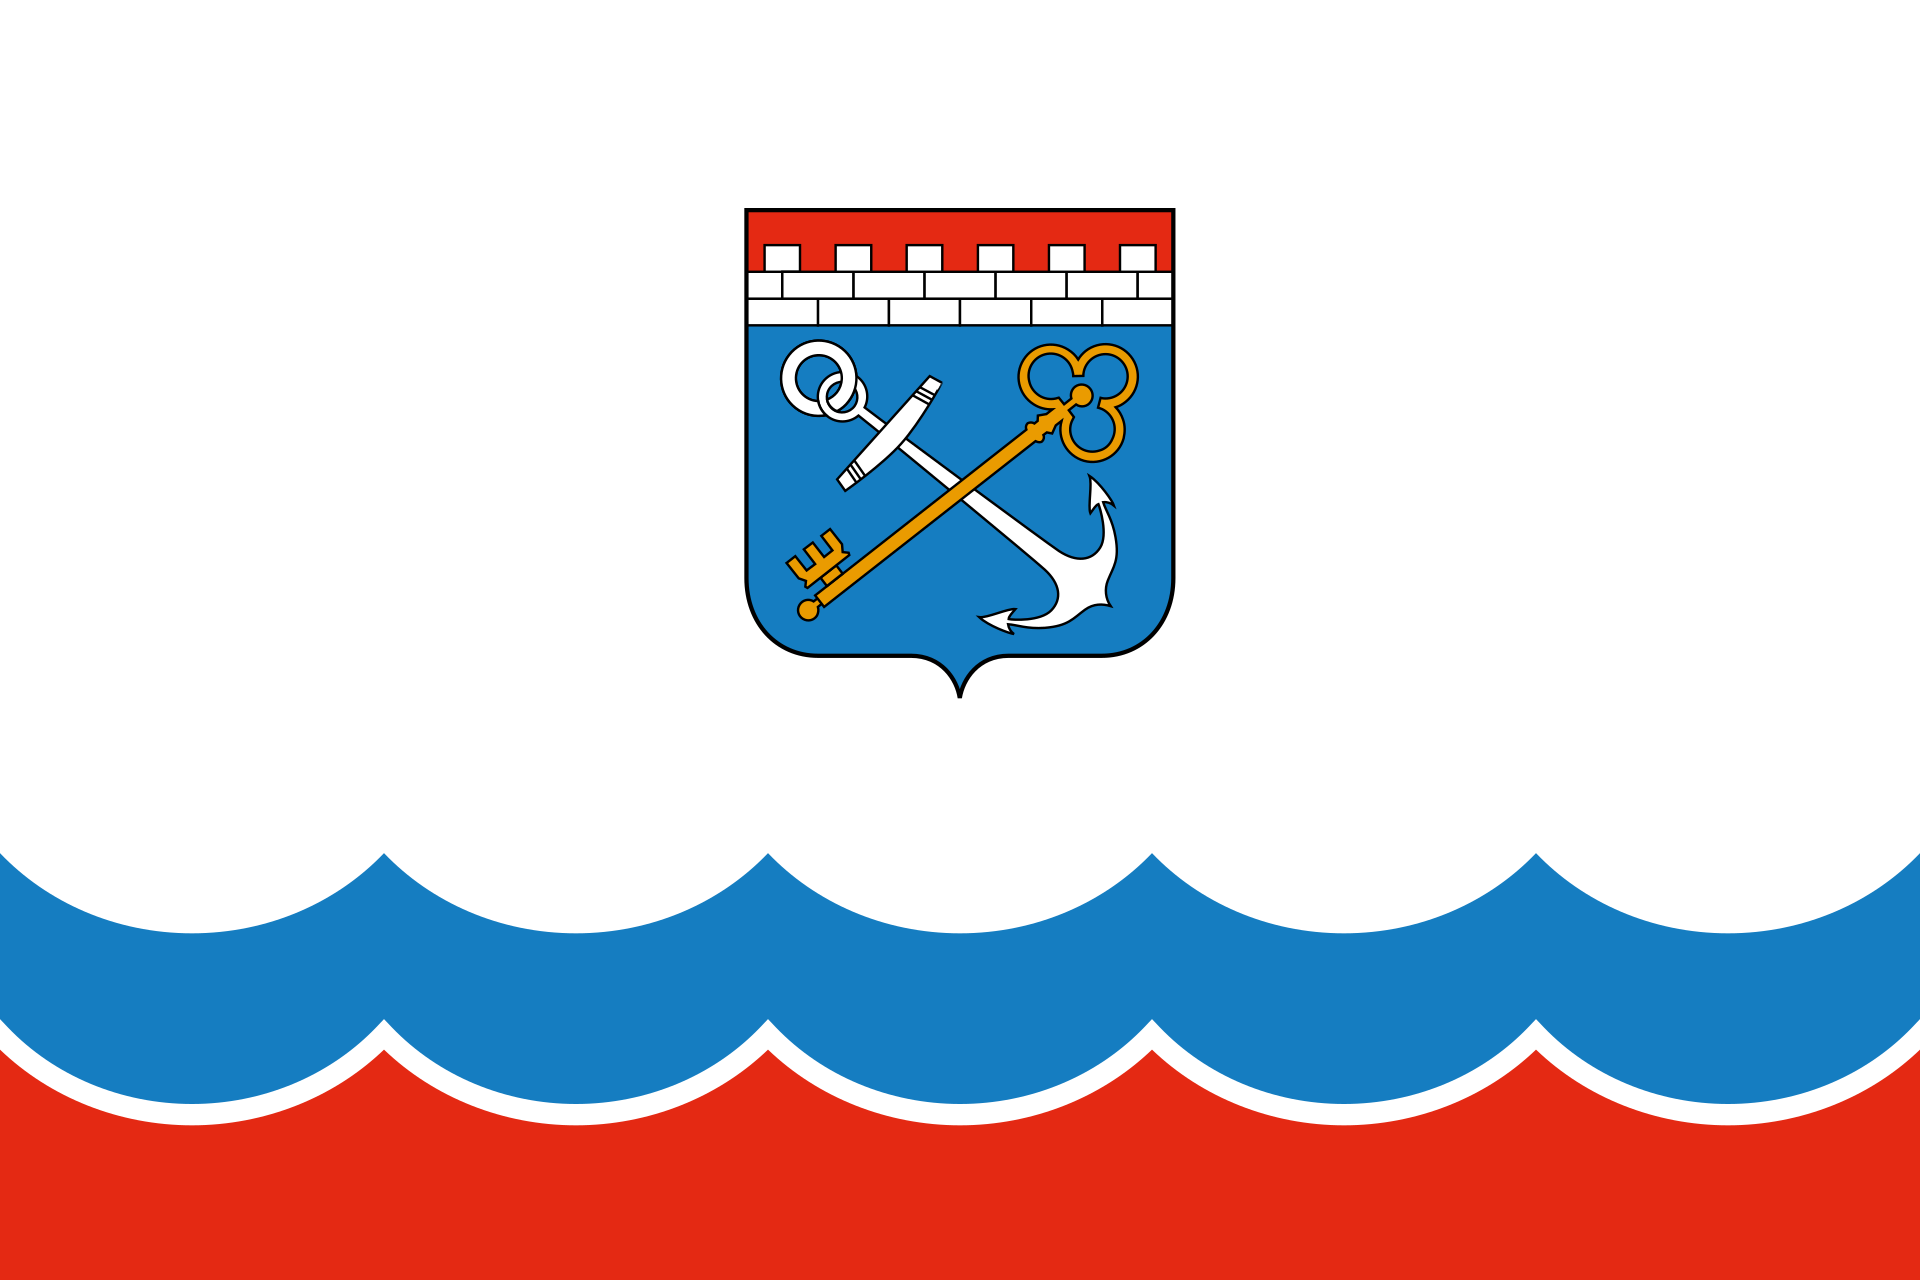
\includegraphics[width=0.8\linewidth]{"chapter/oblast_of_Russia/Flag_of_Leningrad_Oblast.png"}
}
\caption [Флаг Ленинградской области, Россия.]{Флаг Ленинградской области.}%
\label{fig:Flag_of_Leningrad_Oblast}%
\end{marginfigure}
\begin{marginfigure}[0.0cm]
{
	\setlength{\fboxsep}{0pt}%
	\setlength{\fboxrule}{1pt}%
	
\includegraphics[width=0.8\linewidth]{"chapter/oblast_of_Russia/Flag_of_Moscow_oblast.png"}
}
\caption [Флаг Московской области, Россия.]{Флаг Московской области.}%
\label{fig:Flag_of_Moscow_oblast}%
\end{marginfigure}
\begin{marginfigure}[0.0cm]
{
	\setlength{\fboxsep}{0pt}%
	\setlength{\fboxrule}{1pt}%
	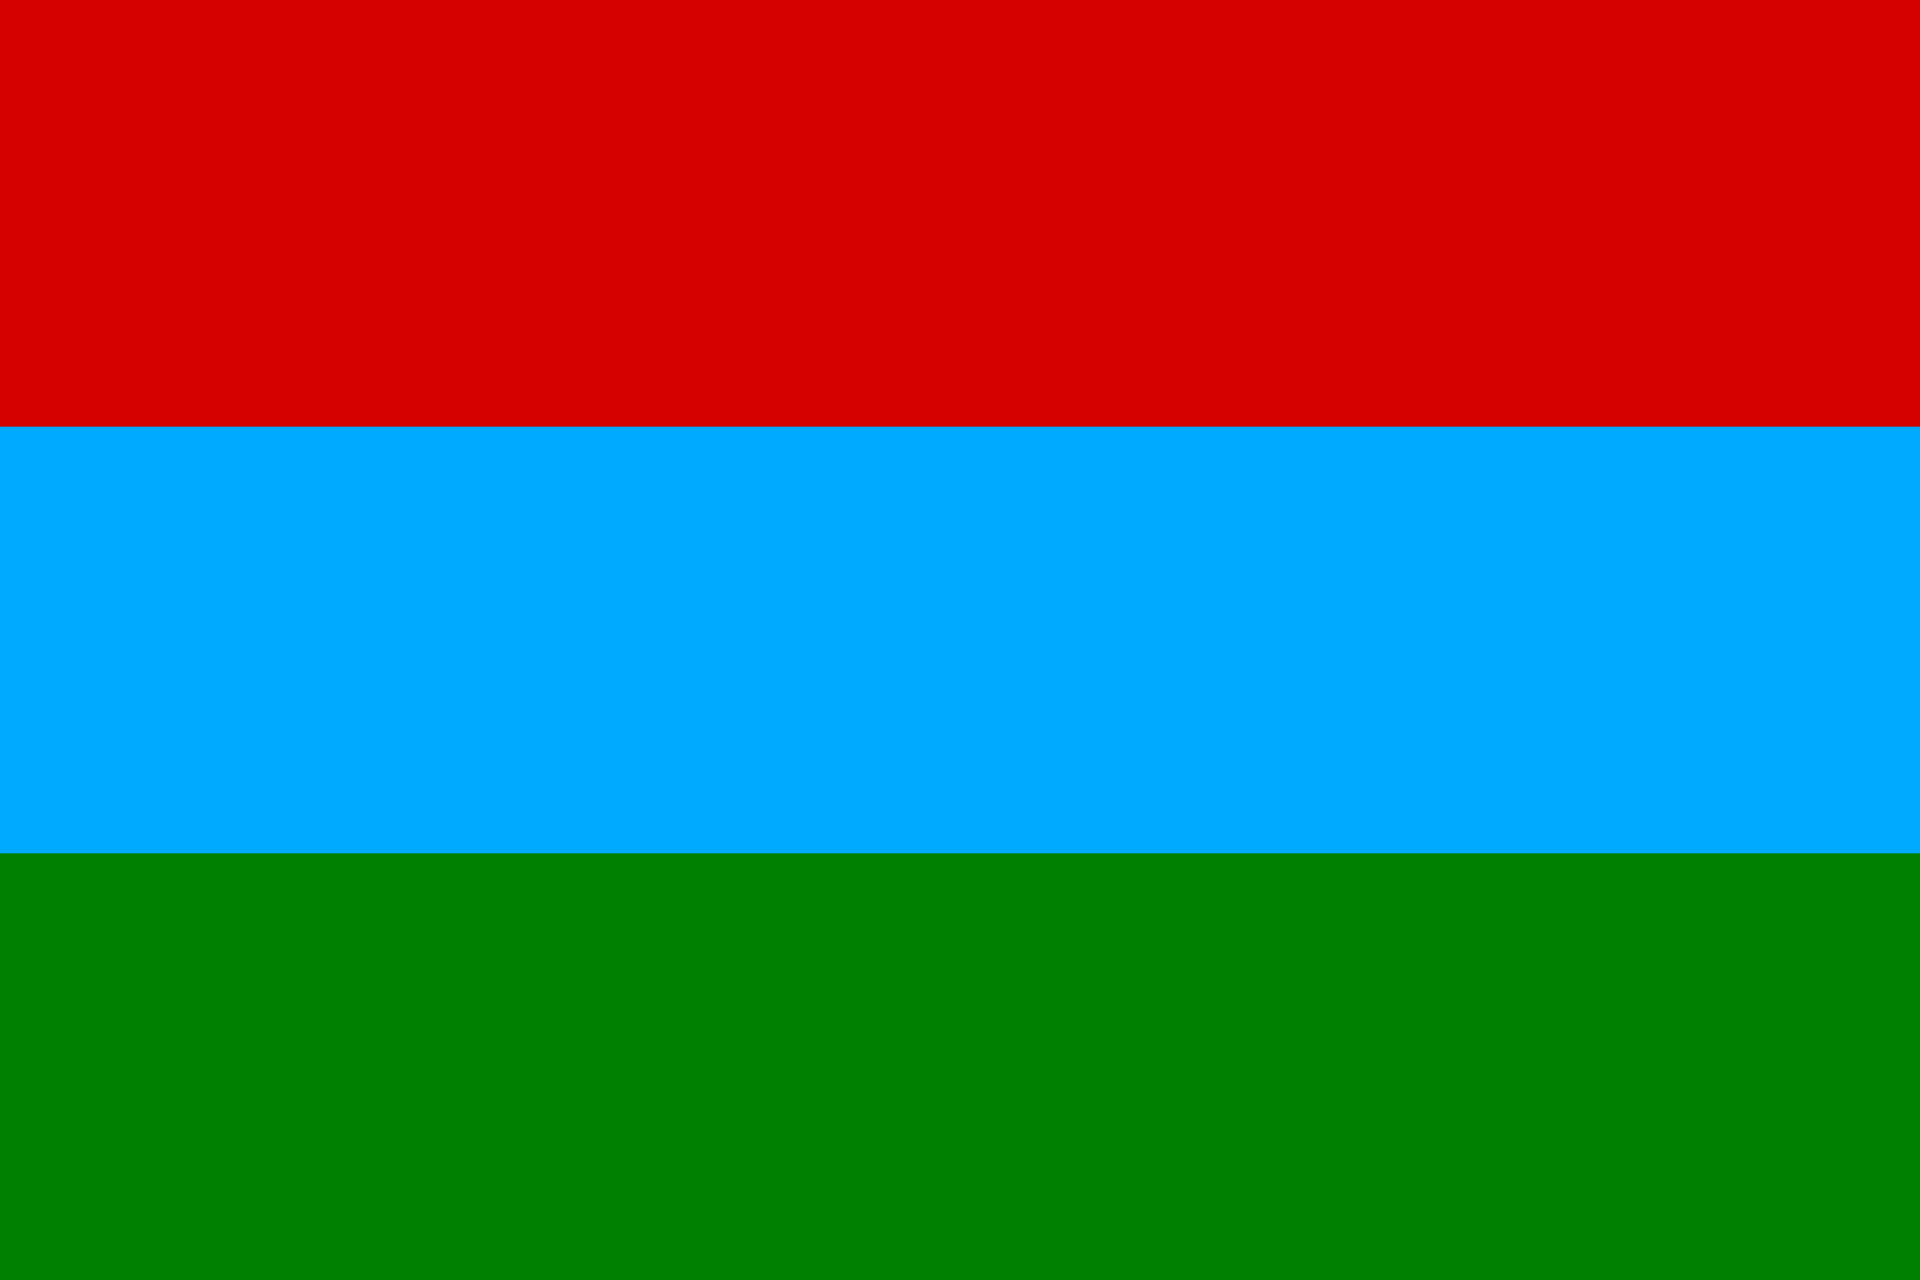
\includegraphics[width=0.8\linewidth]{"chapter/oblast_of_Russia/Flag_of_Karelia.png"}
}
\caption [Флаг Карелии, Россия.]{Флаг Карелии.}%
\label{fig:Flag_of_Karelia}%
\end{marginfigure}
\begin{marginfigure}[0.0cm]
{
	\setlength{\fboxsep}{0pt}%
	\setlength{\fboxrule}{1pt}%
	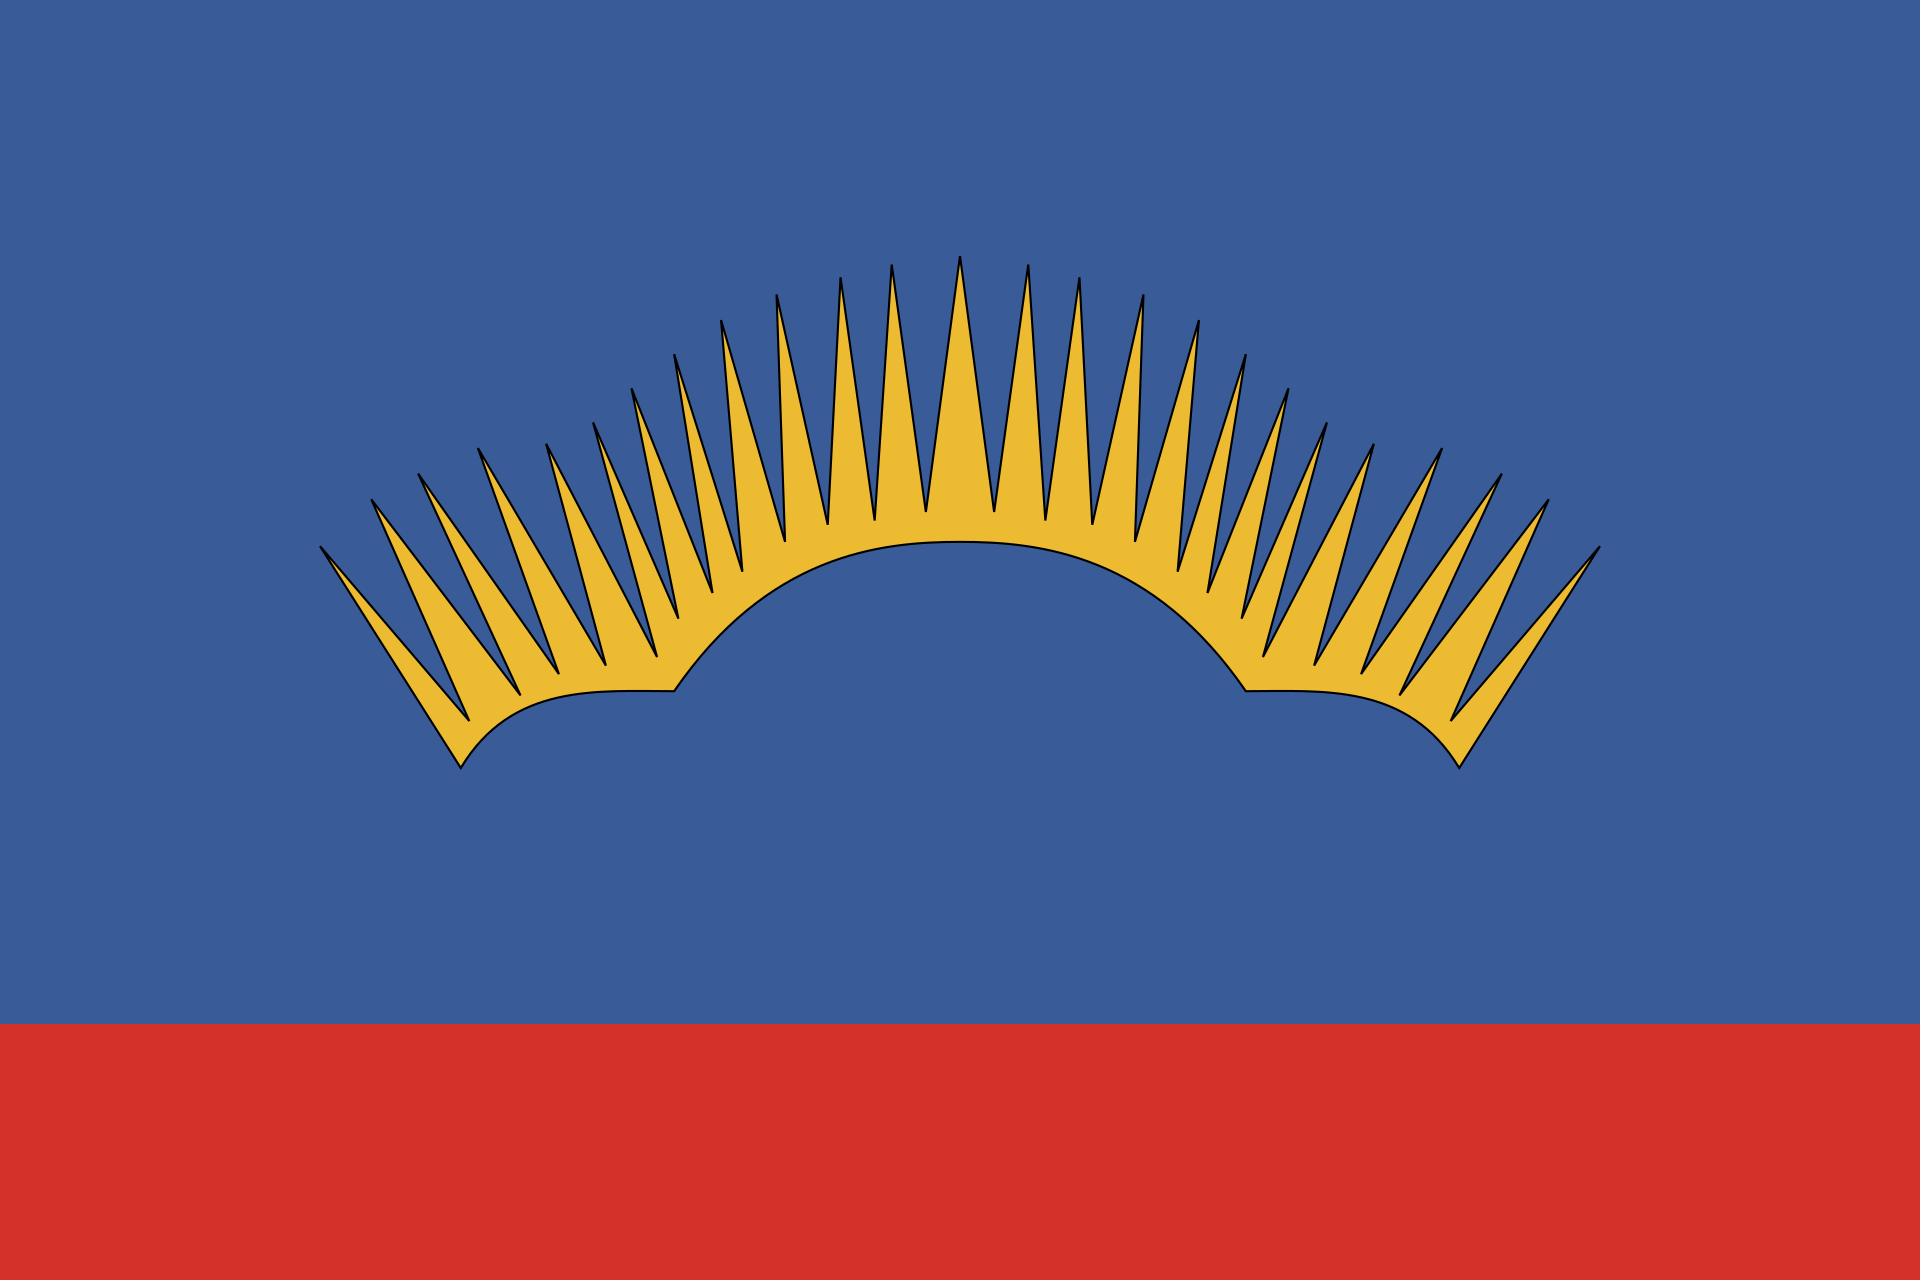
\includegraphics[width=0.8\linewidth]{"chapter/oblast_of_Russia/Flag_of_Murmansk_Oblast.png"}
}
\caption [Флаг Мурманской области, Россия.]{Флаг Мурманской области.}%
\label{fig:Flag_of_Murmansk_Oblast}%
\end{marginfigure}


\lstset{numbers=left, firstnumber=1, frame=single}
\begin{lstlisting}[ language=SPARQL, 
                    caption={\href{https://w.wiki/4DKD}{Граф соседних субъектов России}\protect\footnotemark},
                    label=lst:sharesBorderWith-oblast-of-Russia,
                    texcl 
                    ]
# Graph of subjects of Russia "shares border with". 
#defaultView:Graph
SELECT * WHERE {
 {
   SELECT ?subject ?subjectLabel ?rgb ?subjects ?subjectsLabel 
   WHERE {
     SERVICE wikibase:label 
            { bd:serviceParam wikibase:language "ru". }
     VALUES ?type {
       wd:Q835714 wd:Q41162 wd:Q183342
       wd:Q831740 wd:Q309166 wd:Q184122
     }
     ?subject wdt:P31 ?type.
   }
 }
 UNION
 { ... }
 UNION
 {
   SELECT ?subject ?subjectLabel ?rgb ?subjects ?subjectsLabel 
   WHERE {
     SERVICE wikibase:label 
            { bd:serviceParam wikibase:language "ru". }
     VALUES ?type {
       wd:Q835714 wd:Q41162 wd:Q183342
       wd:Q831740 wd:Q309166 wd:Q184122
     }
     ?subjects wdt:P31 ?type.
     ?oblast wdt:P31 wd:Q835714; wdt:P47 ?subjects.
     
     BIND(IF(?oblast != "", "e87b7b", 
                    IF(?rgb != "", ?rgb, "FFFFFF")) AS ?rgb)
     BIND(IF(?oblast != "", ?oblast, ?subjects) AS ?subject)
     BIND(IF(?oblast != "", ?oblastLabel, 
                    ?subjectsLable) AS ?subjectLable)
   }
 }
}
}
\end{lstlisting}%
\footnotetext{Получено 467 записей в 2017 году 
и 482 записи в 2021 году. Ссылка на SPARQL-запрос: \href{https://goo.su/9xHA}{https://goo.su/9xHA}}

С помощью команды \lstinline|BIND| (строки 31--35) 
записываем значение в~переменную, при условии, что переменная, 
отвечающая за субъекты определённого типа, непустая. 
Например, в строках 31--32 в~переменную \lstinline|?rgb| записывается цвет, 
при условии, что \lstinline|?oblast| не пустая. 
При этом если переменная \lstinline|?rgb| уже содержит значение, 
то его оставляем, чтобы исключить затирание цвета.

Количество полученных записей формируется путём сложения количества соседних территорий для всех субъектов России. Результат работы скрипта~--- это граф, отображающий соседние субъекты. Причём разные типы субъектов имеют вершины разного цвета, например, республики~--- зелёные, а края~--- голубые. Часть графа представлена на рис.~\ref{fig:sharesBorderWith-oblast-of-Russia-Kaliningrad-fig}.

\begin{fullwidth}
\begin{figure*}[h]
	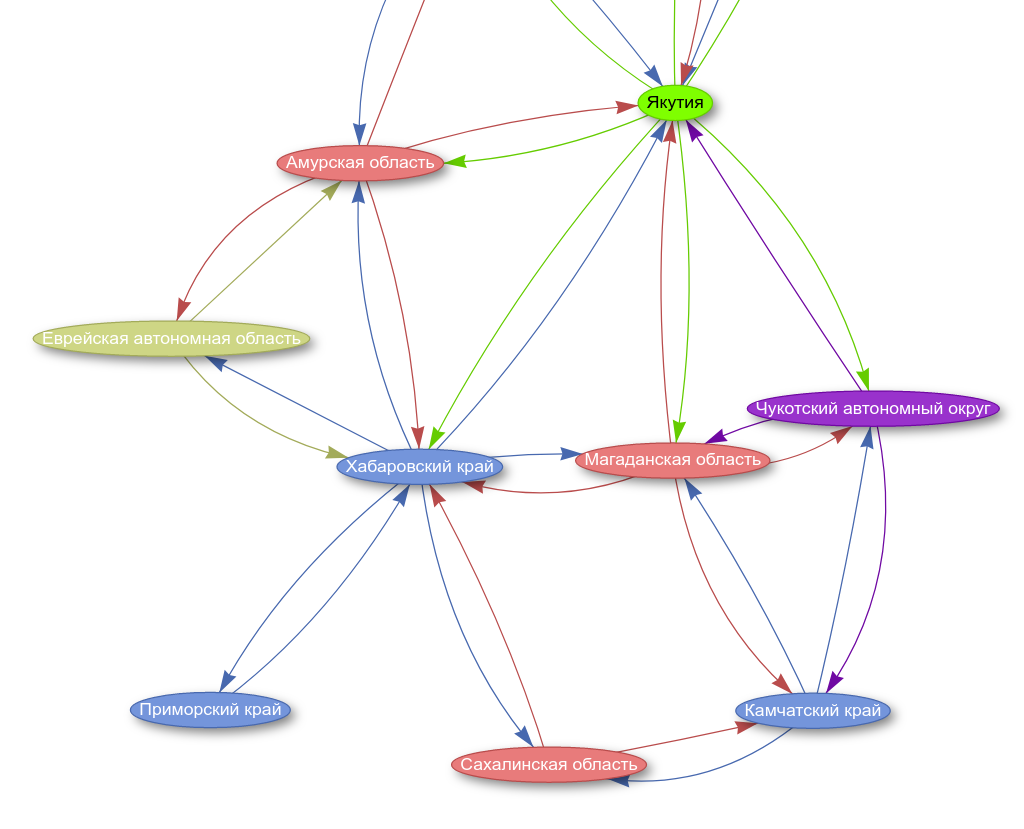
\includegraphics[width=\textwidth]{./chapter/oblast_of_Russia/Graph_Subjects_of_Russia_Siberia_and_the_Far_East_2021.png}
	\caption[Граф субъектов России. Калининград, 2021.]{Регионы России в Сибире и Дальнем востоке на 2021 год. 
    Фрагмент графа соседних субъектов России, построенный по скрипту~\protect\ref{lst:sharesBorderWith-oblast-of-Russia}.
	Республики~--- вершины зелёного цвета (Якутия).
	Автономные округа~--- вершины фиолетового цвета (Чукотский автономный округ).
	Края~--- вершины голубого цвета (Хабаровский край).
	Области~--- вершины розового цвета (Амурская область).
	Автономные области~--- вершины салатового цвета (Еврейская автономная область).}%
      \label{fig:sharesBorderWith-oblast-of-Russia-Kaliningrad-fig}%
\end{figure*} 
\end{fullwidth}

\newpage
Построим карту, на которой цветом обозначены субъекты России, 
граничащие с зарубежными странами. 
Более тёмным цветом обозначены субъекты, у которых большее количество пограничных стран, 
более светлым~--- с меньшим количеством пограничных стран (листинг~\ref{lst:sharesBorderWith-subjects-of-Russia}).

\lstset{numbers=left, firstnumber=1, frame=single}
\begin{lstlisting}[ language=SPARQL, 
                    caption={\href{https://w.wiki/4e82}{Карта субъектов России, граничащих с зарубежными странами}\protect\footnotemark},
                    label=lst:sharesBorderWith-subjects-of-Russia,
                    texcl 
                    ]
# Map of countries around Russia with the number 
# of neighboring regions of Russia
#defaultView:Map\{"hide":["?shape", "?rgb"], "layer": "?regionLabel" \}
SELECT ?region ?regionLabel ?count ?shape ?rgb
{
  {
    SELECT ?region (COUNT(DISTINCT ?country) AS ?count)
    WHERE {
      VALUES ?type {
        wd:Q835714  # oblasts of Russia - 9 neighbours
        wd:Q41162   # republic of Russia - 4
        wd:Q183342  # federal city of Russia - 0 neighbours
        wd:Q831740  # krai of Russia - 4
        wd:Q309166  # autonomous oblast of Russia - 1
        wd:Q184122   # autonomous okrug of Russia - 1
      }
      ?region wdt:P31 ?type.
  
      # Russian region share border with some territory 
      # of foreign country
      ?region wdt:P47 [ wdt:P17 ?country].
      FILTER (?country != wd:Q159) # foreign country is not Russia
    }
    GROUP BY ?region
    HAVING ((COUNT(?country)) > 0)
  }
  ?region wdt:P3896 ?shape.
  BIND(IF(?count = 3 , "6c2eab", 
            IF(?count = 2 , "9b77bf", 
                IF(?count = 1 , "c6b2db", "f5cbce"))) AS ?rgb)
  SERVICE wikibase:label { bd:serviceParam wikibase:language "ru" }  
}
\end{lstlisting}%
\footnotetext{Получено 37 записей в 2021 году. SPARQL-запрос: \href{https://w.wiki/4e82}{https://w.wiki/4e82}}

Результат работы запроса~\ref{lst:sharesBorderWith-subjects-of-Russia} 
представлен на рис.~\ref{fig:MapsharesBorderWithsubjectsofRussia}.

\begin{fullwidth}
\begin{figure*}[h]
	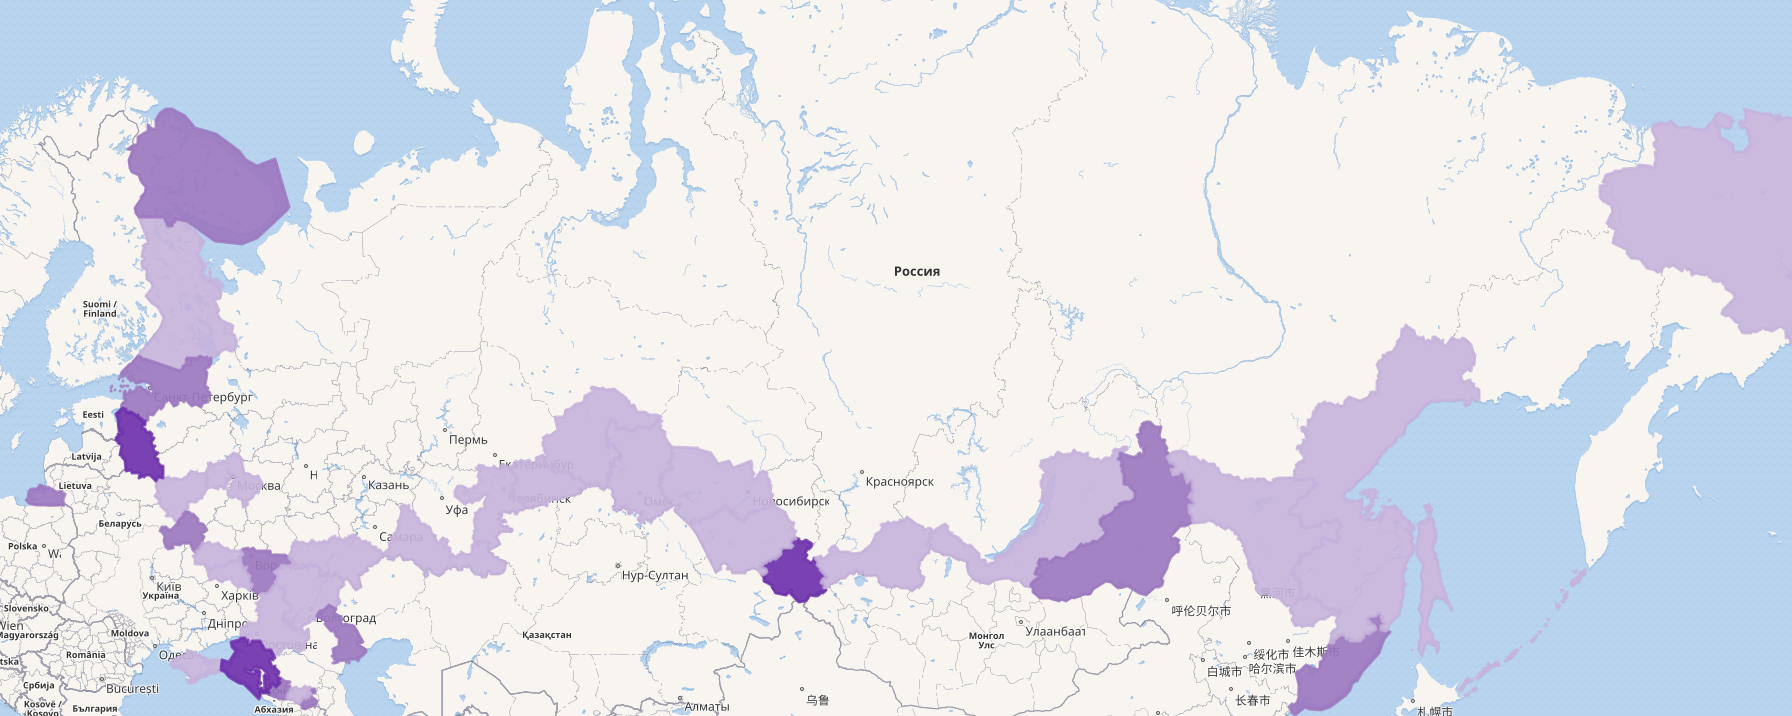
\includegraphics[width=\textwidth]{./chapter/oblast_of_Russia/Maps_of_the_subjects_of_Russia.png}
	\caption[Карта субъектов России, граничащих с зарубежными странами, 2021.]{Карта субъектов России, граничащих с зарубежными странами, 2021. Карта построена с помощью запроса~\protect\ref{lst:sharesBorderWith-subjects-of-Russia}.}%
      \label{fig:MapsharesBorderWithsubjectsofRussia}%
\end{figure*} 
\end{fullwidth}

Построим карту (рис.~\ref{fig:MapsoftheneighbouringstatesofRussia}), 
на которой цветом обозначены зарубежные страны, 
граничащие с субъектами России. 
Более тёмным цветом обозначены страны, у которых большее количество пограничных субъектов России, 
более светлым~--- с меньшим количеством пограничных субъектов России 
(запрос~\ref{lst:Maps_of_the_neighbouring_states_of_Russia}).

\lstset{numbers=left, firstnumber=1, frame=single}
\begin{lstlisting}[ language=SPARQL, 
                    caption={\href{https://w.wiki/4e8T}{Карта зарубежных стран, граничащих с субъектами России}\protect\footnotemark},
                    label=lst:Maps_of_the_neighbouring_states_of_Russia,
                    texcl 
                    ]
# Map of countries around Russia with the number 
# of neighboring regions of Russia
#defaultView:Map\{"hide":["?shape", "?rgb"], "layer": "?countryLabel"\}
SELECT ?country ?countryLabel ?count ?shape ?rgb WHERE {
  {
    SELECT ?country (COUNT(DISTINCT ?region) AS ?count) WHERE {
      VALUES ?type {
        wd:Q835714
        wd:Q41162
        wd:Q183342
        wd:Q831740
        wd:Q309166
        wd:Q184122
      }
      ?region wdt:P31 ?type.
      ?region wdt:P47 [ wdt:P17 ?country].
      FILTER (?country != wd:Q159) # foreign country is not Russia
    }
    GROUP BY ?country
    HAVING ((COUNT(?region)) > 0 )
  }
  ?country wdt:P3896 ?shape.
  BIND(IF(?count > 9 , "4B0082", 
        IF(?count > 5 , "800080", 
         IF(?count > 2 , "8B008B", 
          IF(?count > 1 , "9400D3", 
           IF(?count > 0 , "DA70D6", "f5cbce"))))) AS ?rgb)
  SERVICE wikibase:label {bd:serviceParam wikibase:language "ru".}
}
\end{lstlisting}%
\footnotetext{Получено 15 записей в 2021 году. 
SPARQL-запрос: \href{https://w.wiki/4e8T}{https://w.wiki/4e8T}}

\begin{fullwidth}
\begin{figure*}[h]
	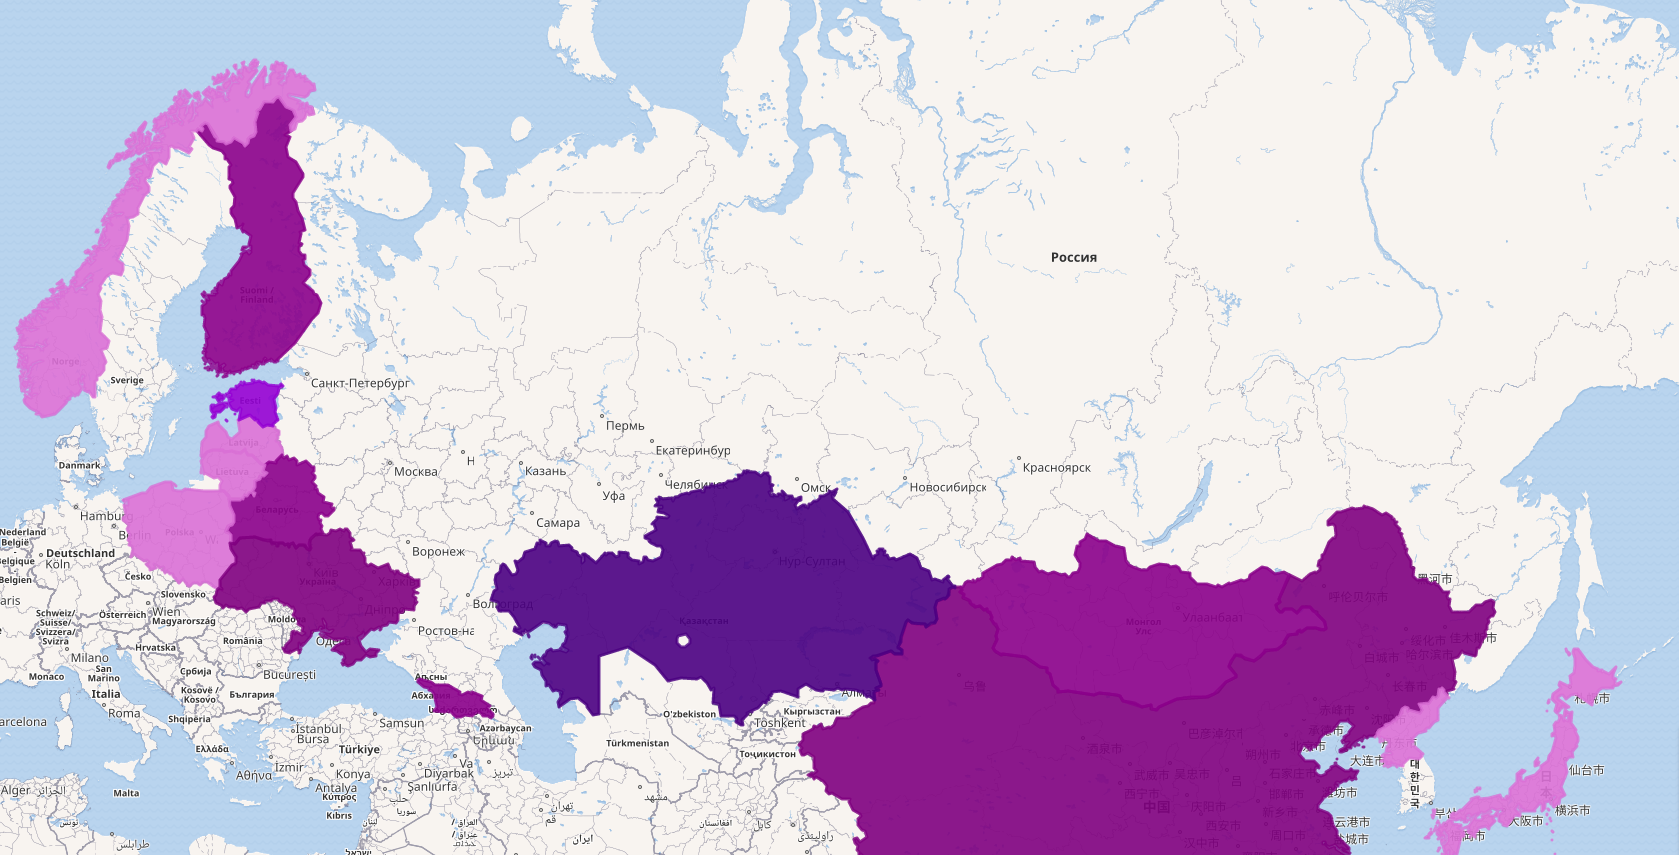
\includegraphics[width=\textwidth]{./chapter/oblast_of_Russia/Maps_of_the_neighbouring_states_of_Russia.png}
	\caption[Карта зарубежных стран, граничащих с субъектами России, 2021.]{Карта зарубежных стран, граничащих с субъектами России, 2021. Карта построена с помощью запроса~\protect\ref{lst:Maps_of_the_neighbouring_states_of_Russia}.}%
      \label{fig:MapsoftheneighbouringstatesofRussia}%
\end{figure*} 
\end{fullwidth}



\subsection{Полнота Викиданных}

С помощью запроса~\ref{lst:sharesBorderWith-empty-oblast-of-Russia} 
построим список субъектов России 
с~пустым свойством \wdProperty{47}{``shares border with''} (граничит с), 
то есть попробуем найти такие субъекты, которые ни с кем не граничат.

\label{question:q_subjects_of_Russia_2}
\marginnote{Какие из перечисленных далее субъектов входят в состав Российской Федерации, а какие~--- нет:
\begin{itemize}
  \item Республика Адыгея;
  \item Камчатский край;
  \item Читинская область;
  \item Чукотский автономный округ.
\end{itemize}
См. ответ \ref{answer:subjects_of_Russia_2} на с.~\pageref{answer:subjects_of_Russia_2}.
}

\marginnote[4.0cm]{Получено 0 записей в 2017 году и 0 записей в 2021 году. SPARQL-запрос: \href{https://w.wiki/4bHb}{https://w.wiki/4bHb}}
\lstset{numbers=left, firstnumber=1, frame=single}
\begin{lstlisting}[ language=SPARQL, 
                    caption={\href{https://w.wiki/4bHb}{Список субъектов РФ с пустым свойством \wdProperty{47}{``shares border with''}}\protect\footnotemark},
                    label=lst:sharesBorderWith-empty-oblast-of-Russia,
                    texcl 
                    ]
# List of `subjects of Russia`~without `shares border with`. 
SELECT 
    ?subject ?subjectLabel 
    ?sharesBorderWith ?sharesBorderWithLabel
WHERE
{
  VALUES ?type {wd:Q835714   # Oblast of Russia
                wd:Q41162    # Republic of Russia
                wd:Q183342   # Federal city of Russia
                wd:Q831740   # Krai of Russia
                wd:Q309166   # Autonomus oblast of Russia
                wd:Q184122}  # Autonomus okrug of Russia
  ?subject wdt:P31 ?type.
  
  FILTER EXISTS {?subject wdt:P17 wd:Q159; wdt:P31 ?type}
  
  MINUS { ?subject  wdt:P47 [] } . #Shares border with 
  SERVICE wikibase:label { bd:serviceParam wikibase:language "ru"}
}
\end{lstlisting}%
%\footnotetext{Получено 0 записей в 2017 году и 0 записей в 2021 году. SPARQL-запрос: \href{https://w.wiki/4bHb}{https://w.wiki/4bHb}}

С помощью команды \lstinline|FILTER| (строка 15 запроса~\ref{lst:sharesBorderWith-empty-oblast-of-Russia}) 
исключаем объекты, которые не находятся на территории России. 
Затем с помощью команды \lstinline|MINUS| (строка 17) удаляем из рассмотрения объекты, 
у которых свойство \wdProperty{47}{<<граничит с>>} заполнено.

Таким образом, на Викиданных для всех субъектов России свойство \wdProperty{47}{<<граничит с>>} заполнено.



\section{Численность населения по субъектам Российской Федерации}

Обозначим на карте субъекты Российской Федерации, 
разделив их на шесть групп по количеству населения. 
Субъектам, принадлежащим одной группе, будет соответствовать на карте один цвет.

Для запроса~\ref{lst:map} нам потребуются свойства \wdProperty{625}{<<координаты>>} 
и \wdProperty{1082}{<<численность населения>>}.

\index{График!Map!Карта населения России}
\begin{lstlisting}[ language=SPARQL, numbers=none,
                    caption={\href{https://w.wiki/4bHe}{Карта населения России}\protect\footnotemark},
                    label=lst:map,
                    texcl 
                    ]
# Map of population of subjects of Russia
#defaultView:Map
SELECT DISTINCT ?subject ?subjectLabel ?population ?coord ?layer
{
  {
    { ?subject wdt:P31 wd:Q835714 } UNION  # Oblast of Russia
    { ?subject wdt:P31 wd:Q41162 } UNION  # Republic of Russia
    { ?subject wdt:P31 wd:Q183342 } UNION  # Federal city of Russia
    { ?subject wdt:P31 wd:Q831740 } UNION  # Krai of Russia
    { ?subject wdt:P31 wd:Q309166 } UNION # Autonomus oblast 
                                                        of Russia
    { ?subject wdt:P31 wd:Q184122 } # Autonomus okrug of Russia
  }   
  ?subject wdt:P625 ?coord; wdt:P1082 ?population.
  
  BIND(
    IF(?population < 500000, "< 500000",
    IF(?population < 1000000, "500000 - 1000000",
    IF(?population < 3000000, "1000000 - 3000000",
    IF(?population < 8000000, "3000000 - 8000000",
    IF(?population < 10000000, "8000000 - 10000000",
    "> 10000000")))))
    AS ?layer).
  
  SERVICE wikibase:label { bd:serviceParam wikibase:language "ru"}
}
ORDER BY ?population
\end{lstlisting}%
\footnotetext{Получено \num{85} записей в 2017 году и \num{86} записей в 2021 году. Ссылка на SPARQL-запрос: \href{https://w.wiki/4bHe}{https://w.wiki/4bHe}}

Результат работы запроса~\ref{lst:map} представлен на рис.~\ref{fig:SubjectsRussiaMap}.

\begin{fullwidth}
\begin{figure*}[h]
	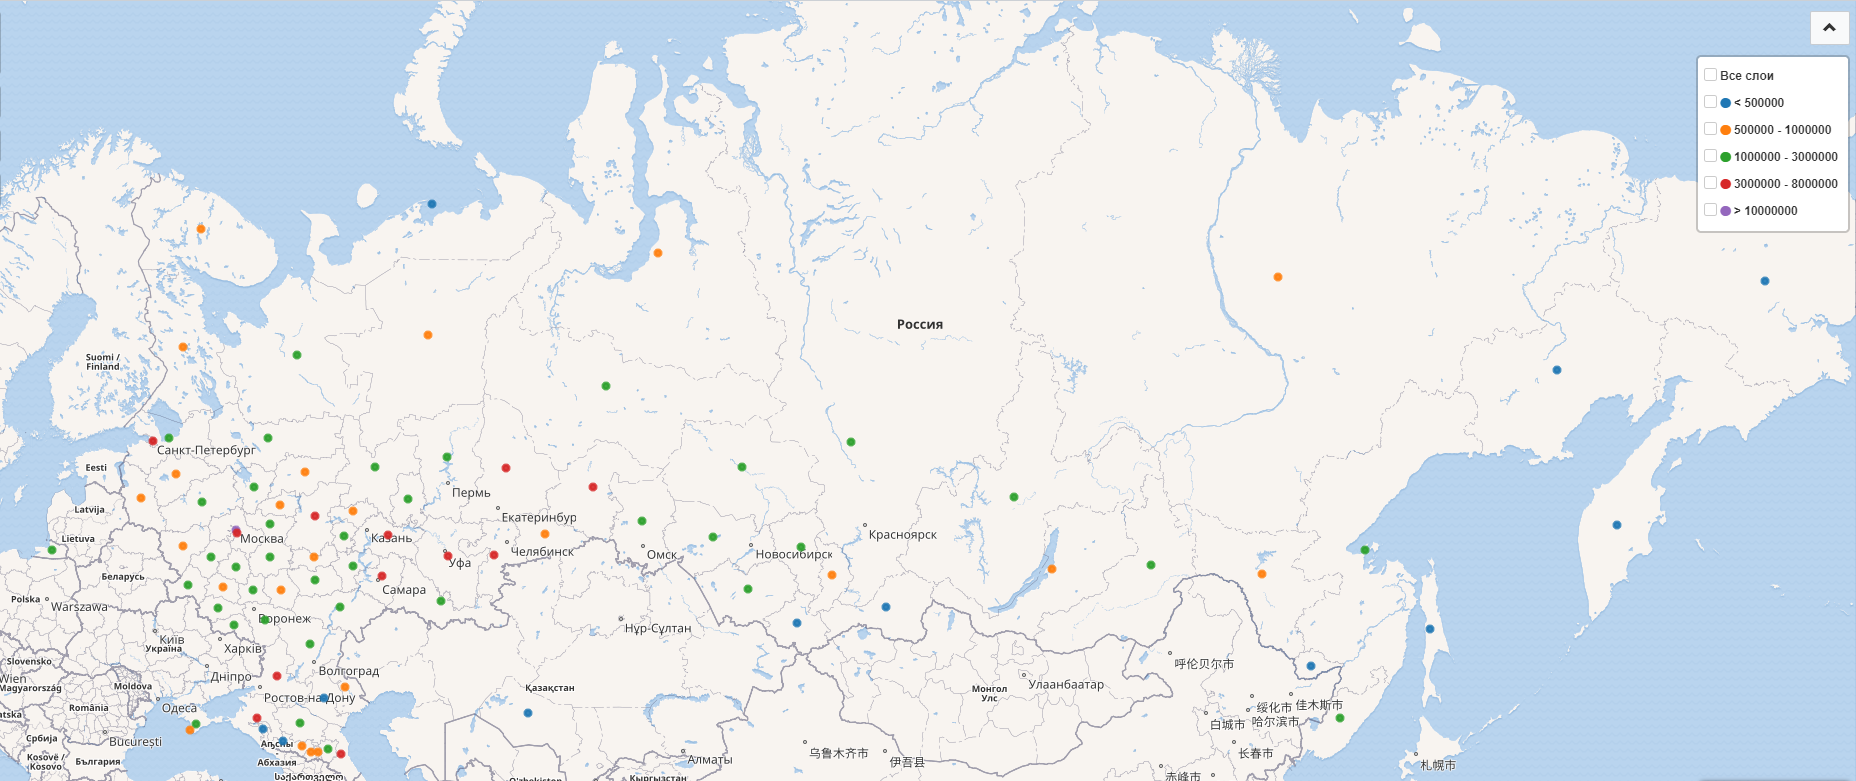
\includegraphics[width=\textwidth]{./chapter/oblast_of_Russia/SubjectsRussia_Map_with_legend_RU.png}
	\caption[Карта численности населения по субъектам России, 2021.]{Карта численности населения по субъектам России, 2021. Субъекты разделёны на шесть групп по количеству населения и отмечены разными цветами в зависимости от группы, в которую субъект входит. Карта построена с помощью запроса~\protect\ref{lst:map}.}%
      \label{fig:SubjectsRussiaMap}%
\end{figure*} 
\end{fullwidth}

